\documentclass{IEEEtaes}
% First draft. Not submission-ready. Do not treat template sample
% authors, DOI, volume or 2020 dates as this manuscript.
\usepackage{cite}
\usepackage{amsmath,amssymb}
\usepackage{tikz}
\usetikzlibrary{positioning}
\usepackage[ruled,vlined,linesnumbered]{algorithm2e}
\usepackage[T1]{fontenc}
\usepackage{textcomp}

\SetKwRepeat{Do}{do}{while}

% Shared manuscript macros. Do not alter accepted algorithm semantics.
\newcommand{\IFpred}{\texttt{IF-PRED-OBS}}
\newcommand{\IFhist}{\texttt{IF-HIST-UPDATE}}
\newcommand{\IFobs}{\texttt{IF-OBS-INTERPRET}}
\newcommand{\IFsel}{\texttt{IF-SELECT-ADMIT}}
\newcommand{\IFexec}{\texttt{IF-EXECUTE-RECORD}}
\newcommand{\IFprep}{\texttt{IF-PREP-RECOVER}}
\newcommand{\IFeq}{\texttt{IF-EQUIV}}
\newcommand{\IFres}{\texttt{IF-RESOURCE-STOP}}

% Visible evidence placeholder. Never used to draw fake data.
\newcommand{\phboxhigh}[3]{%
  \begin{center}
  \fbox{%
    \begin{minipage}{0.92\linewidth}
      \vspace{28mm}
      \centering
      \textbf{Placeholder #1} (#2)\\[0.4em]
      {\small #3}\\[0.3em]
      {\scriptsize Data are not obtained. This framed panel reserves a single-column result figure. It is not a curve, a mean, or a significance test.}
      \vspace{28mm}
    \end{minipage}}
  \end{center}
  \label{ph:#1}%
}
\newcommand{\phbox}[3]{%
  \begin{center}
  \fbox{%
    \begin{minipage}{0.92\linewidth}
      \vspace{1.15em}
      \centering
      \textbf{Placeholder #1} (#2)\\[0.35em]
      {\small #3}\\[0.25em]
      {\scriptsize Data are not obtained. This box reserves layout. It is not a result.}
      \vspace{1.15em}
    \end{minipage}}
  \end{center}
  \label{ph:#1}%
}


\title{CL-TAV: Closed-Loop Test--Analysis Verification for ARINC 615A Data Loading under Timing Uncertainty}

\author{Author~Name~\IEEEmembership{Membership pending}
\thanks{Manuscript received date pending. Authors, affiliations, funding and
IEEE membership are institutional inputs (AUTH-AUTHORS, AUTH-AFFIL, AUTH-FUND)
and are not fabricated. Corresponding author, ORCID and clearance remain
pending. AI disclosure remains incomplete (AUTH-AI): system name PENDING-USER;
sections/figures/code touched PENDING-USER; verification duty remains with the
authors. This sentence does not fulfill IEEE AESS AI disclosure
(https://ieee-aess.org/publications/transactions-aes/author-information).
No AI system is an author.}
\thanks{Affiliation pending (AUTH-AFFIL).}}

\begin{document}
\maketitle

\begin{abstract}
ARINC 615A data loading must be judged under declared timers, file identities
and measurement uncertainty. A fixed test suite that never uses residual
ambiguity, or an analysis that never issues a later legal operation, can leave
detection and isolation incomplete. This paper specifies Closed-Loop
Test--Analysis Verification (CL-TAV): a charged session that predicts current
observation classes, selects an exclusive TEST, Prep, Recover or Admit action,
interprets timing with a shared uncertainty reference, and updates a
single-fault candidate set only from a select-time snapshot. Unknown-effect
\texttt{ERROR} is not implementation FAIL. Confirmed-not-sent leaves the known
summary unchanged. The bound protocol model remains UPLOAD and INFORMATION;
ARINC 645 identity is bound for triggered leaves, while integrity capabilities
stay unestablished. Four comparison arms and three registered experiment
families are defined. Confirmatory measurements are not yet obtained;
improvement percentages are therefore not reported. The draft is a journalized
method paper, not a solver implementation and not a certification argument.
\end{abstract}

\begin{IEEEkeywords}
Avionics, data loading, conformance testing, fault diagnosis, timing
uncertainty, closed-loop verification.
\end{IEEEkeywords}

\section{Introduction}
\label{sec:intro}

Airborne software loaders exchange INFORMATION and UPLOAD traffic under declared
timers, file identities and operator actions~\cite{arinc615a3}. A single missed
or late acknowledgement, a mismatched Load File, or an unresolved integrity
check can be read as a protocol failure, a measurement artefact, or an
unconfirmed injection. The engineering problem is therefore not only whether a
fixed suite eventually reports PASS, but whether a later legal action can be
chosen from residual ambiguity under a finite resource.

Requirements-based generation organises stimuli from obligations~\cite{yang2025}.
Conformance relations such as \emph{ioco} generate tests from labelled
transition systems~\cite{tretmans1996}. FSM coverage and mutant killing select
discriminating sequences~\cite{chow1978,fujiwara1991,petrenko2016,jia2011}.
Those methods address detection or selection. They do not, as stated, close an
observation--update--select loop that treats preparatory actions, unknown-effect
\texttt{ERROR}, and exclusive finite stops as first-class objects. That is a
scope comparison, not a claim that those methods cannot be extended.

This paper specifies Closed-Loop Test--Analysis Verification (CL-TAV) for
ARINC~615A data loading under timing uncertainty. The question to be answered
experimentally is: under a declared protocol, fault domain, measurement
uncertainty and resource mode, does test--analysis feedback improve verdict
reliability and isolation at an interpretable cost? Two propositions are
evaluated, not asserted as established results:
\begin{itemize}
\item C1: uncertainty-aware interpretation, timing verdicts and compatible
candidate update stay mutually consistent.
\item C2: residual ambiguity feeds the next action with explicit resource,
Prep/Recover, \texttt{ERROR} and stop rules.
\end{itemize}

The evaluation plan uses four arms (CL-T, CL-A, CL-TA, CL-LOOP) and three
registered families (DETECT, LOCATE, ABLATION). Confirmatory numbers are not
available; Section~\ref{sec:results} reserves the result layout.
\phbox{PH-ABS-RESULT}{AUTHOR-INPUT / EXPERIMENT-RESULT}{Abstract and conclusion
improvement statements remain empty until registered runs exist.}

Section~\ref{sec:related} states the problem objects.
Section~\ref{sec:arch} separates protocol CRS, tool requirements and the two
machines.
Section~\ref{sec:method} gives the loop and conditional properties.
Section~\ref{sec:setup} freezes the comparison contract.
Sections~\ref{sec:results}--\ref{sec:concl} hold results, limits and the
unfinished experimental sentence.
The supplement records ALG-CLTAV-05/06/07, wrappers and the S0--S10 map.
The paper Algorithm numbers are display labels; the stable repository IDs are
unchanged.

\section{Related Work and Problem Formulation}
\label{sec:related}

\subsection{Selective comparison}
Table~\ref{tab:related} compares nearby methods on five attributes required by
CL-RQ1--CL-RQ3. ``Not the stated object'' means the cited paper does not
develop that contract; it is not a proof of impossibility. Full-text access
gaps are listed as PH-LIT-ACCESS rather than turned into negative capability
claims.

\begin{table}[!t]
\caption{Selective comparison. Entries are about the cited paper's stated object.}
\label{tab:related}
\centering
\begin{tabular}{@{}p{0.20\columnwidth}p{0.70\columnwidth}@{}}
\hline
Work & Stated object relative to this paper \\
\hline
Tretmans~\cite{tretmans1996} & Implementation relation and test generation from LTS; not residual isolation under a charged verification budget. \\
Chow~\cite{chow1978}, Fujiwara~\textit{et al.}~\cite{fujiwara1991} & FSM covering sequences; no measurement-uncertainty partition shared by prediction and interpretation. \\
Petrenko~\textit{et al.}~\cite{petrenko2016} & Constraint solving and mutant killing for FSMs. \\
Jia and Harman~\cite{jia2011} & Mutation adequacy, not session-level Prep/Recover or \texttt{ERROR} versus IUT FAIL. \\
Yang~\textit{et al.}~\cite{yang2025} & Requirements-based generation survey; obligation coverage is not a closed diagnostic loop. \\
Li~\textit{et al.}~\cite{li2021} & Model-based testing of networked applications; not ARINC 615A integrity residuals. \\
Alur and Dill~\cite{alur1994} & Timed automata theory used as a timing vocabulary, not as an implemented solver. \\
\hline
\end{tabular}
\end{table}

\phbox{PH-LIT-ACCESS}{LITERATURE-ACCESS}{If a later negative comparison needs a
paywalled method detail that cannot be obtained through the institution, that
citation stays unused for the specific denial.}

\subsection{Verification objects}
The implementation under test (IUT) is a 615A data-loading endpoint. The bound
protocol model remains UPLOAD and INFORMATION~\cite{arinc615a3}. Research
coverage of FIND, DOWNLOAD and conditional AFDX is a CRS fact; it is not
implemented behaviour and not an experimental arm.

The first-version candidate set is
\(H_0=\{h_{\mathrm{normal}}\}\cup H_{\mathrm{single}}\).
An observable summary \(q\) is known or unknown. Observation classes are
projected onto the current \(H\). Measurement uncertainty follows the GUM
vocabulary~\cite{jcgm100,jcgm106}: a declared conservative outer set \(U\), not
an estimated physical error model. Resource is exactly one mode:
BUDGET\((c_{\min},B)\) or ROUNDS\((K_{\max})\), never a logical OR of both.

A 615A-triggered 645 identity and semantic bind exists for CRC, check-value and
naming leaves~\cite{arinc6451}. Four integrity capabilities remain
not established. Stop-645 therefore names a remaining 645-dependent obligation,
not a missing file.

\section{System Engineering and Verification Architecture}
\label{sec:arch}

Protocol CRS, tool requirements and experiment requirements stay in separate
layers. Row count does not prove a method. A concrete owned trace is source
unit \texttt{SU-ARINC-615A-3-SECTION-6-3-2-}\allowbreak
\texttt{SEQUENCE-CHART-A-E007-7726A816FFE7}
\(\to\) CRS-M1-00365/00366/00367 \(\to\) LUR write-order constraint \(\to\)
planned Test/Analysis verification case \(\to\) later tool module. The IDs are
real bound-M1 identifiers. \texttt{satisfy}/\texttt{verify} in the SysML view
are model relations, not executed verification. No standard figure is reprinted.

Two machines must not be merged. \(M_{\mathrm{sess}}\) selects from
\(S\subseteq A(q)\), charges once, updates \(H\) and returns a named stop.
\(M_{\mathrm{prot}}\) is the UPLOAD/INFORMATION black box. Execute issues a
stimulus and obtains a raw execution record. Interpretation, not the network
port, produces the compatible class \(I_z\) and hypothesis survivors.

\begin{figure}[!ht]
\centering
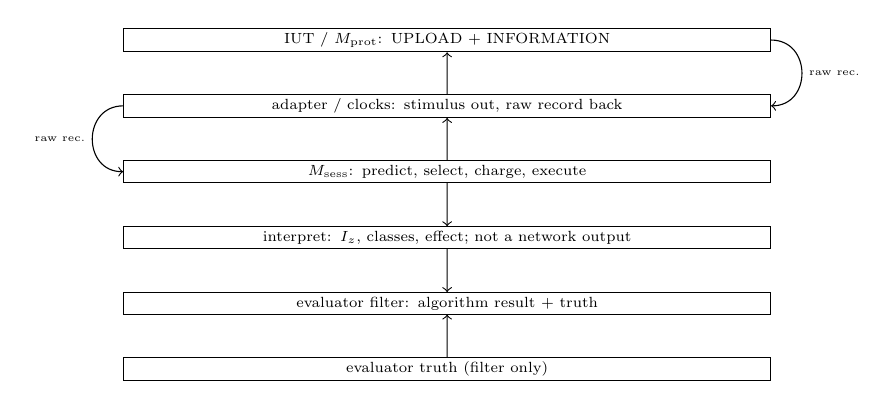
\begin{tikzpicture}[scale=0.76,transform shape,font=\scriptsize,box/.style={draw,align=center,inner sep=2pt,text width=0.88\columnwidth}]
\node[box] (iut) at (0,4.4) {IUT / \(M_{\mathrm{prot}}\): UPLOAD + INFORMATION};
\node[box] (adp) at (0,3.3) {adapter / clocks: stimulus out, raw record back};
\node[box] (sess) at (0,2.2) {\(M_{\mathrm{sess}}\): predict, select, charge, execute};
\node[box] (interp) at (0,1.1) {interpret: \(I_z\), classes, effect; not a network output};
\node[box] (filt) at (0,0.0) {evaluator filter: algorithm result + truth};
\node[box] (truth) at (0,-1.1) {evaluator truth (filter only)};
\draw[->] (sess) -- (adp);
\draw[->] (adp) -- (iut);
\draw[->] (iut.east) to[out=0,in=0,looseness=1.6] node[right,font=\tiny] {raw rec.} (adp.east);
\draw[->] (adp.west) to[out=180,in=180,looseness=1.6] node[left,font=\tiny] {raw rec.} (sess.west);
\draw[->] (sess) -- (interp);
\draw[->] (interp) -- (filt);
\draw[->] (truth) -- (filt);
\end{tikzpicture}
\caption{Context derived from FIG-CL-TAV-01/07. Stimulus and raw records share
ports. Truth enters only the evaluator filter, never select, predict, history
or execute.}
\label{fig:arch}
\end{figure}

Expanded CRS leaves do not add FIND or DOWNLOAD transitions to
\(M_{\mathrm{prot}}\).
\phbox{PH-IMPL-KERNEL}{IMPLEMENTATION-DETAIL}{Core estimators, pairing solvers
and the history representation remain interface contracts and are not deployed.}

\section{CL-TAV Method}
\label{sec:method}

\subsection{Notation and assumptions}
S0--S10 are logical duties, not line numbers or protocol states. The decision
index \(k\), the billed charge count and the retry counter are distinct.
Assignment is \(\leftarrow\). SessionContext \(\Gamma\) is the unique session
state; HistoryHandle \(\eta\) carries whole-history compatibility.
\(q_{\mathrm{used}}\) (\texttt{qUsedAtSelect}) is frozen after the final action
and before charge or execute. A later confirmed summary is a different field.
Effect classes are \texttt{CONFIRMED-NOT-SENT} and \texttt{UNKNOWN-EFFECT}.
The former leaves \(q\) and compatible history unchanged and still counts the
retry. The latter marks \(\eta\) conservative-unknown and assigns UNKNOWN.
Unconfirmed Recover stays UNKNOWN and joins the same retry policy.
PredictionGapError is TEST-scoped: empty current classes do not block an
eligible Recover or Prep.

\subsection{Overall closed loop}
Algorithm~\ref{alg:cltav-01} is the compact top-level session (stable ID
ALG-CLTAV-01). It is not an executable engine and selects no solver. The
supplement typesets ALG-CLTAV-05/06/07; wrappers ALG-CLTAV-02/03/04 stay there.
TEST, Prep, Recover and Admit are exclusive. Charge occurs once. History
advances from the select-time snapshot. If no P-stop fires, the next iteration
returns to the entry stop gate.

% Compact display of ALG-CLTAV-01. Same duties and interfaces as the
% authoritative module; not a second control algorithm.
\begin{algorithm}[t]
\caption{CL-TAV top-level session (paper Alg.~1 = ALG-CLTAV-01)}
\label{alg:cltav-01}
\SetKwInput{KwIn}{Require}
\SetKwInput{KwOut}{Ensure}
\KwIn{\(H_0=\{h_{\mathrm{normal}}\}\cup H_{\mathrm{single}}\); \(\Gamma\); \(\eta\); one mode BUDGET\((c_{\min},B)\) xor ROUNDS\((K_{\max})\); library \(L\); uncertainty \(U\)}
\KwOut{stop class, final \(H\), \(\eta\), trace; singleton \(h_{\mathrm{normal}}\) is not protocol PASS}
\textsc{Initialize}; \While{true}{
  \lIf{\IFres{} already decided}{\Return that stop}
  \(\textit{pred}\leftarrow\textsc{PredictCurrent}\) via \IFpred\;
  \(\textit{dec}\leftarrow\textsc{SelectAndAdmit}\) via \IFsel\;
  \lIf{\(\textit{dec}\) is EXIT or SPEC-ERROR}{\Return its reason}
  freeze snapshot \(\xi\) (action, \(q_{\mathrm{used}}\), history version, classes)\;
  charge \(\xi\) once; \(\textit{er}\leftarrow\) \IFexec\((\Gamma,\xi)\)\;
  \(z\leftarrow\textsc{InterpretOutcome}\) via \IFobs{} and ALG-CLTAV-06\;
  \(\delta\leftarrow\textsc{ResolveOutcome}\); adopt returned \((\Gamma,\eta,z)\)\;
  \lIf{\(\delta=\texttt{STOP}\)}{\Return reason}
  \lIf{\(\delta=\texttt{RETRY}\)}{\textbf{continue}}
  \If{\(z\) has valid \(I_z\) or a confirmed successor summary}{
    commit via \IFhist{} from \(\xi\), not from the post-effect \(q\)\;
  }
  \lIf{a P-stop is set}{\Return it}
}
\end{algorithm}


\subsection{Interpretation, compatibility and selection}
Prediction and interpretation share one uncertainty reference \(U\). Classes
project onto current \(H\). A prediction gap is not scored as remaining
\(|H|\). Compatible update intersects \(H\) with a currently valid class;
\texttt{ERROR} and identity Prep/Recover do not exclude \(H\). Instance
ownership and pairing are single results: an ambiguous pair is
\texttt{ERROR}, not IUT FAIL. Timing uses the accepted three-valued treatment
with distinct closed and open horizons (ALG-CLTAV-06).

Selection scores only affordable distinguishing TESTs. The one-step score is
the worst remaining-candidate count on currently valid nonempty classes. Empty
selectable \(S\) is never \(\arg\min\). If no distinguishing TEST remains,
Prep is preferred to Recover when eligible. Confirmed Recover is the sole
writer of KNOWN. S9 is the sole commit of a confirmed successor summary.

\subsection{Conditional properties}
The following are the accepted short arguments, not global optimality or
physical correctness.

\noindent\textbf{Monotonicity.} A valid update satisfies \(H_{k+1}\subseteq H_k\).
\texttt{ERROR} and identity Prep/Recover leave \(H\) unchanged. An in-domain
singleton is not protocol PASS.

\noindent\textbf{Retention.} If the true hypothesis is in \(H_0\), a
whole-history path exists, the observation outer set is conservative, the
realized \(I_z\) contains the true observation, and ownership/pairing are
valid, then a valid update retains the true hypothesis. Out-of-domain faults
may still mimic an in-domain survivor.

\noindent\textbf{One-step minimax.} On a nonempty finite selectable set the
chosen TEST is a least element of
\((s(t),\mathrm{cost}(t),\mathrm{id})\). This is not a global policy.

\noindent\textbf{Termination.} Every charged TEST, Prep, Recover and
\texttt{ERROR} spends the selected mode, so the number of billed executions is
at most \(\lfloor B/c_{\min}\rfloor\) or \(K_{\max}\). Wall-clock return of
each wait still needs its own timeout argument; this draft does not claim
those timeouts are implemented.

Named stops remain exclusive: Empty, Singleton, 645, Equivalent, Budget, and
retry-cap Stop-Error. Stop-Error is not Stop-Budget. A confirmed-not-sent
adapter outcome does not rewrite \(q\) to UNKNOWN. An unknown effect must not
be read back as the previous KNOWN summary. Unconfirmed Recover with
\(R_{\max}=1\) and remaining budget is Stop-Error. An executed empty candidate
set is Stop-Empty.

The compact display is a duty-preserving view of ALG-CLTAV-01. Reviewers
compare it with the accepted module; this paper does not introduce a second
loop. Core kernels remain interface-bound and unimplemented.

\section{Experimental Setup and Evaluation Protocol}
\label{sec:setup}

The comparison contract is the existing experiment plan. It is not altered
here. Four arms share the same action pool, fault domain and charged resource
mode:

\begin{itemize}
\item CL-T: predetermined tests; no analysis feedback into the next test.
\item CL-A: analysis on a fixed observation set; no further legal operations.
\item CL-TA: collect with a frozen policy, then analyse; the loop does not close.
\item CL-LOOP: the CL-TAV session; the update chooses the next action.
\end{itemize}

Independent truth is evaluator-only. It never enters \IFsel, \IFpred, \IFhist{}
or \IFexec. Injection planned is not injection confirmed. Unconfirmed,
invalid, equivalent and abstain records are not detection PASS or FAIL.
Denominators always include the attempt set and the answered subset.

\begin{figure}[!t]
\centering
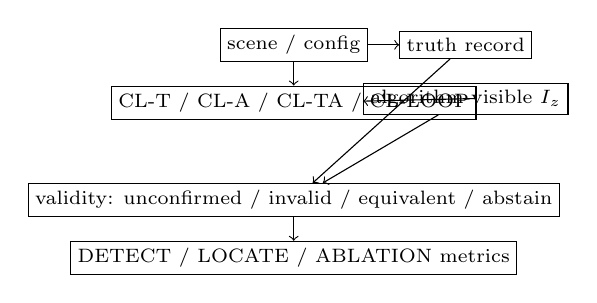
\begin{tikzpicture}[font=\scriptsize,box/.style={draw,align=center,inner sep=2.5pt},arr/.style={->}]
\node[box] (scene) {scene / config};
\node[box,right=4mm of scene] (truth) {truth record};
\node[box,below=3mm of scene] (arms) {CL-T / CL-A / CL-TA / CL-LOOP};
\node[box,below=3mm of truth] (obs) {algorithm-visible \(I_z\)};
\node[box,below=8mm of arms] (valid) {validity: unconfirmed / invalid / equivalent / abstain};
\node[box,below=3mm of valid] (met) {DETECT / LOCATE / ABLATION metrics};
\draw[arr] (scene) -- (arms);
\draw[arr] (scene) -- (truth);
\draw[arr] (arms) -- (obs);
\draw[arr] (obs) -- (valid);
\draw[arr] (truth) -- (valid);
\draw[arr] (valid) -- (met);
\end{tikzpicture}
\caption{Experiment architecture derived from FIG-CL-TAV-09. Truth reaches
metrics only after the validity filter.}
\label{fig:exp}
\end{figure}

DETECT asks whether CL-LOOP increases missed detections or converts
equality-timing into false FAIL relative to CL-T under the same budget. LOCATE
asks whether the surviving set shrinks without excluding the confirmed true
fault. ABLATION disables feedback, timing partitions or cost accounting
separately. Sample size, seeds and effect thresholds remain a named decision
gap; they are not chosen for writing convenience.

\phbox{PH-STAT-N}{PUBLICATION-DECISION}{Numeric \(n\), repeats and interval
method freeze at confirmatory registration, not in this draft.}

Platforms, devices and live loaders are planned. Software Ethernet experiments,
when later run, will not prove AFDX hardware determinism or certification.

\section{Results}
\label{sec:results}

No effect direction, percentage or superiority is reported.

\subsection{CL-RQ2: verdict reliability}
\begin{figure}[!t]
\centering
\phboxhigh{PH-RES-DETECT}{EXPERIMENT-RESULT}{Separate cells, not one shared
denominator: (i) attempt coverage on all registered attempts; (ii) refusal
rate (abstain/INCONCLUSIVE/unconcluded among attempts); (iii) conditional
error on the answered subset; (iv) miss and false-FAIL on the detection
denominator after invalid and equivalent faults are removed. Abstain is not a
PASS/FAIL. Source: EXP-CLTAV-DETECT.}
\caption{Reserved detection panel. Not a result.}
\label{fig:res-detect}
\end{figure}

\subsection{CL-RQ2: isolation}
\begin{figure}[!t]
\centering
\phboxhigh{PH-RES-LOCATE}{EXPERIMENT-RESULT}{Cells: final \(|H|\), true-fault
exclusion, refusal, charged resource. Denominator: confirmed in-domain
injections. Out-of-domain faults are reported separately. Singleton
\(h_{\mathrm{normal}}\) is not protocol PASS. Source: EXP-CLTAV-LOCATE.}
\caption{Reserved localization panel. Not a result.}
\label{fig:res-locate}
\end{figure}

\subsection{CL-RQ3: cost and sensitivity}
\begin{table}[!t]
\caption{Reserved ablation cells. CL-A is computation-only; N/A cells are not
silent omissions. FIND-abort waiver is a forbidden control.}
\label{tab:res-ablation}
\centering
\scriptsize
\begin{tabular}{@{}lcccc@{}}
\hline
Cell & CL-T & CL-A & CL-TA & CL-LOOP \\
\hline
Charged projection & \(c_{\mathrm{acq}}\) & \(c_{\mathrm{comp}}\) & split & actual \\
No-feedback contrast & yes & N/A & yes & reference \\
Prep/Recover uncharged & if run & N/A & if run & contrast \\
Interval vs point stamp & --- & --- & --- & contrast \\
FIND-abort waiver & forbidden & forbidden & forbidden & forbidden \\
\hline
\end{tabular}
\end{table}
\phbox{PH-RES-ABLATION}{EXPERIMENT-RESULT}{Table~\ref{tab:res-ablation} uses the
registered ablation factors, not a generic ``disable cost accounting.'' Complete
when parent DETECT/LOCATE cells exist on the same scenes.}

\section{Discussion and Limitations}
\label{sec:disc}

The first-version domain is a declared single-fault \(H_0\), one-step
selection, a bound UPLOAD/INFORMATION model, and notation-only architecture
views. Out-of-domain faults may remain compatible with an in-domain survivor.
A remaining \(\{h_{\mathrm{normal}}\}\) is not a protocol PASS. Obtaining
ARINC~645 and binding triggered leaves does not close the four integrity
capabilities.

Engineering work that is not done includes the core estimators, an executable
verification engine, Project Configuration and confirmatory runs. Those
absences are unfinished work, not method impossibility.

\phbox{PH-RES-INTERPRET}{EXPERIMENT-RESULT}{Discussion of measured gains or
losses waits for the reserved result panels. No placeholder may be read as a
neutral or negative experimental outcome.}

Transfer beyond Ethernet laboratory loaders, and any certification argument,
remain open (historical RQ6).

\section{Conclusion}
\label{sec:concl}

CL-TAV specifies a charged observation--update--select session for ARINC~615A
data loading under declared uncertainty and one resource mode. The main-text
loop keeps interpretation, compatible update and exclusive stops consistent
with the accepted algorithm package. Experimental answers to CL-RQ2 and
CL-RQ3 are not available.
\phbox{PH-CONC-RESULT}{EXPERIMENT-RESULT}{The concluding experimental sentence
stays empty until PH-RES-DETECT, PH-RES-LOCATE and PH-RES-ABLATION are
cleared by registered runs.}

This draft is not submission-ready, not an implemented solver, and not
capability establishment.


\bibliographystyle{IEEEtaes}
\bibliography{references}

\end{document}
